\lecture{21}{8 maggio 2024}
\subsection{Formule di Fresnel}
Oggi studiamo la relazione fra polarizzazione e passaggio fra due mezzi ottici distinti.
\begin{figure}[H]
	\centering
	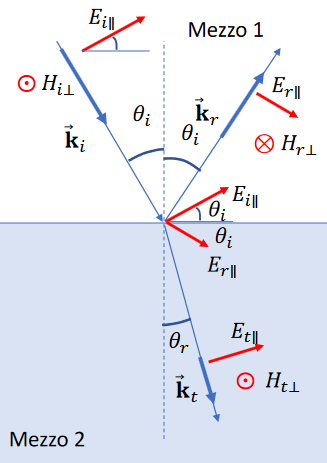
\includegraphics[width=0.4\textwidth]{screenshots/2024-05-08-09-15-56.png}
\end{figure}
Se l'incidenza dell'onda non è normale, allora nello spazio esiste un piano definito dalla normale alla superficie e dalla direzione di moto dell'onda. La componente del campo elettrico che sta su questo piano ha proprietà di riflessione e rifrazione diverse da quelle della componente normale a tale piano (per ora studiamo la componente del campo elettrico parallela al piano d'incidenza e insieme la componente perpendicolare del campo magnetico). I versi in figura sono stati messi coerentemente con quanto fatto ieri per \(\theta _i \to 0\), sia per il campo elettrico che per il campo magnetico (N.B.: queste sono tutte scelte arbitrarie!).
Le considerazioni fatte ieri sulla circuitazione valgono anche in questo caso:
\begin{equation}
	E_{i \parallel} \cos (\theta _i) + E_{r \parallel} \cos (\theta _i) = E_{t \parallel} \cos (\theta _r)
\end{equation}
Il campo magnetico invece è perpendicolare al piano incidente e parallelo alla superficie di separazione, quindi ho la relazione già studiata:
\begin{equation}
	H_{i \perp } - H_{r \perp } = H_{t \perp } \implies n1 E_{i \parallel} - n_1 E_{r \parallel} = n_2 E_{t \parallel}
\end{equation}
Pongo
\begin{align}
	\alpha &= \frac{\cos (\theta _r)}{\cos (\theta _i)} &
	\beta &= \frac{n_2}{n_1}
\end{align}
da cui si ha
\begin{equation}
	\begin{cases}
		E_{i \parallel} + E_{r \parallel} = \alpha E_{t \parallel}\\
		E_{i \parallel} - E_{r \parallel} = \beta E_{t \parallel}	
	\end{cases}
\end{equation}
Si ottengono così le formule di Fresnel per il campo elettrico parallelo:
\begin{figure}[H]
	\centering
	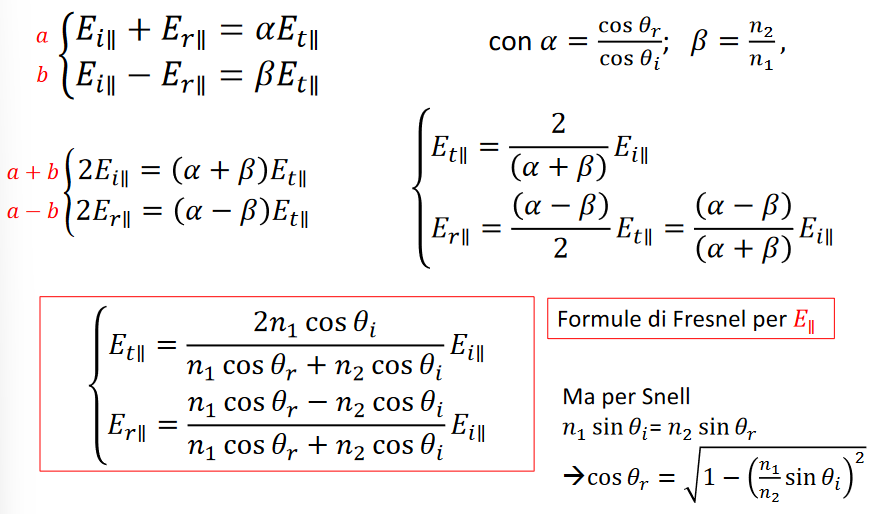
\includegraphics[width=0.5\textwidth]{screenshots/2024-05-08-09-32-20.png}
\end{figure}
Disegniamo quello che sta accadendo:
\begin{figure}[H]
	\centering
	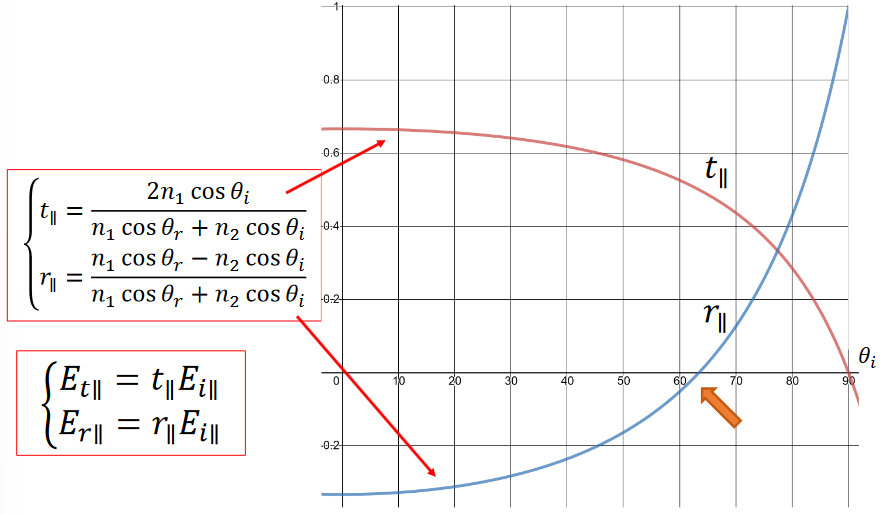
\includegraphics[width=0.5\textwidth]{screenshots/2024-05-08-09-33-56.png}
\end{figure}
Sapendo che \(I= \quotient{1}{Z} \langle E ^{2}  \rangle \) e ponendo \(R_\parallel = r_\parallel ^{2} \), si ottiene immediatamente che \(I_{r \parallel} = R_\parallel I_{i \parallel}\). Posto invece \(T_\parallel = \frac{4 \alpha \beta }{(\alpha + \beta )^{2} }\), si ha \(I_{t \parallel} = T_\parallel I_{i \parallel} \quotient{\cos (\theta _i)}{\cos (\theta _r)} \).
\begin{figure}[H]
	\centering
	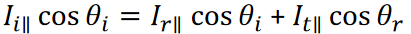
\includegraphics[width=0.4\textwidth]{screenshots/2024-05-08-09-38-56.png}
\end{figure}
Non si conserva l'intensità. Per fortuna la fisica è salva, perché l'importante è che si conservi l'energia. L'intensità non si conserva perché varia la superficie su cui è distribuita la potenza dell'onda.

Studiamo ora il caso del campo elettrico perpendicolare al piano d'incidenza e il campo magnetico parallelo al piano d'incidenza.
\begin{figure}[H]
	\centering
	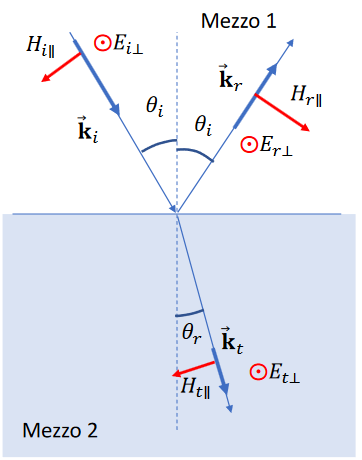
\includegraphics[width=0.4\textwidth]{screenshots/2024-05-08-09-40-42.png}
\end{figure}
Per la continuità del campo elettrico usiamo la formula dell'incidenza normale: \(E_{i \perp } + E_{r \perp } = E_{t\perp } \). Per il campo magnetico invece vale un ragionamento analogo a prima, da cui si ottiene \(H_{i\parallel }\cos (\theta _i) - H_{r\parallel } \cos (\theta _i) = H_{t\parallel } \cos (\theta _r)   \). Pongo \(\alpha, \beta \) come prima e trovo
\begin{figure}[H]
	\centering
	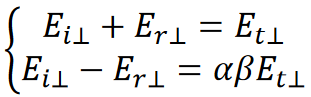
\includegraphics[width=0.2\textwidth]{screenshots/2024-05-08-09-44-26.png}
\end{figure}
Svolgendo nuovamente i calcoli come prima troviamo le formule di Fresnel per il campo elettrico perpendicolare:
\begin{figure}[H]
	\centering
	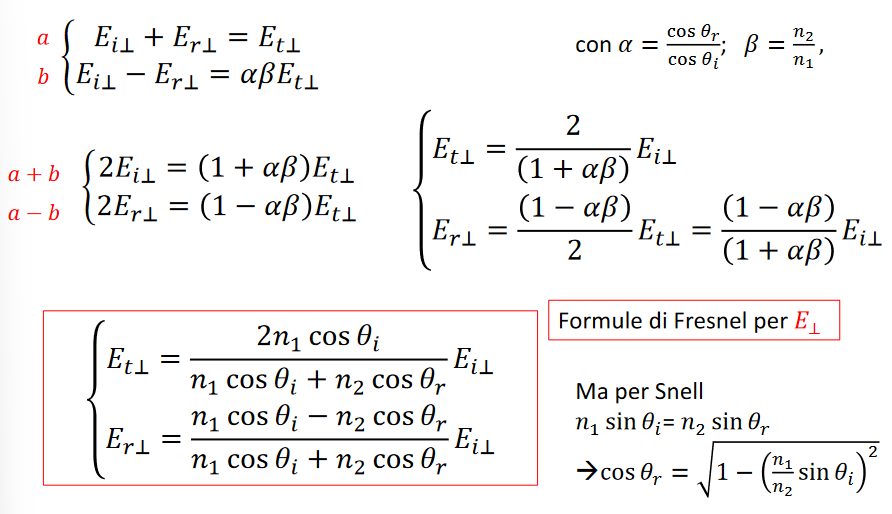
\includegraphics[width=0.5\textwidth]{screenshots/2024-05-08-09-45-58.png}
\end{figure}
Disegniamo quello che sta succedendo:
\begin{figure}[H]
	\centering
	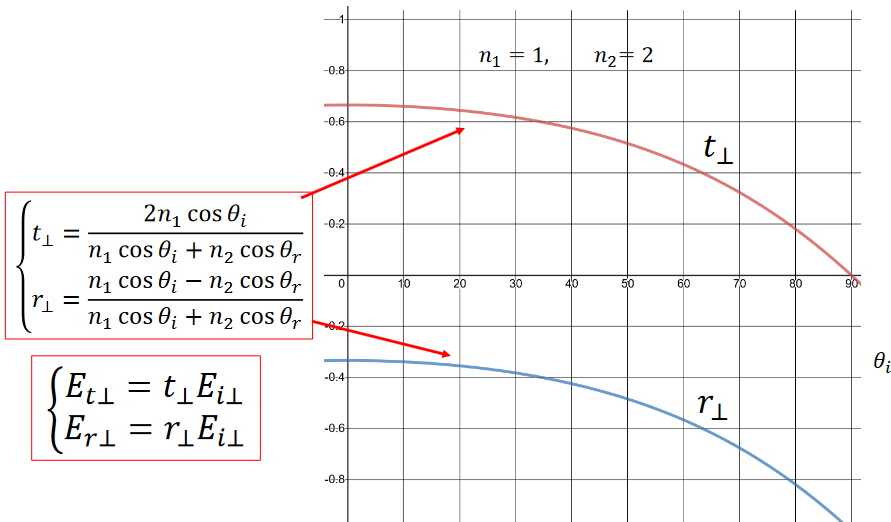
\includegraphics[width=0.5\textwidth]{screenshots/2024-05-08-09-47-02.png}
\end{figure}
Anche sull'intensità facciamo lo stesso identico calcolo di prima. Chiamiamo \(R_{\perp } = r_{\perp }^{2}   \) e \(T_{\perp } = \frac{4 \alpha \beta }{(1 + \alpha \beta )^{2} } \). Si ha che \(I_{r\perp } = R_{\perp }I_{i\perp }   \) e \(I_{t\perp }= T_{\perp }I_{i\perp } \frac{\cos (\theta _i)}{\cos (\theta_r)}  \), per cui risulta:
\begin{figure}[H]
	\centering
	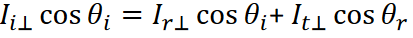
\includegraphics[width=0.3\textwidth]{screenshots/2024-05-08-09-50-30.png}
\end{figure}
Stesso discorso di prima sull'energia.

Caso per caso devo capire quale è la componente perpendicolare e quale la componente parallela dell'onda incidente.

\paragraph{Angolo di Brewster}
% TODO: recupera tutto questo discorso da slide
Abbiamo visto che c'è un angolo per cui \(r_{\parallel } =0	\). Questo equivale a dire che \(n_1 \cos (\theta _r) = n_2 \cos (\theta _i)\). Dalla legge di Snell, questa relazione è verificata quando \(\theta _i + \theta _r = \frac{\pi}{2}\). In questo caso \(\theta _i = \theta _B\) "angolo di Brewster". La luce riflessa è totalmente polarizzata.
\begin{formula}
	[Angolo di Brewster]
	Dall'equazione che definisce l'angolo di Brewster e dalla legge di Snell si ricava che:
	\begin{equation}
		\tan (\theta _B) = \frac{n_2}{n_1}
	\end{equation}
\end{formula}